\documentclass{article}



\usepackage{arxiv}

\usepackage[utf8]{inputenc} % allow utf-8 input
\usepackage[T1]{fontenc}    % use 8-bit T1 fonts
\usepackage{hyperref}       % hyperlinks
\usepackage{url}            % simple URL typesetting
\usepackage{booktabs}       % professional-quality tables
\usepackage{amsfonts}       % blackboard math symbols
\usepackage{nicefrac}       % compact symbols for 1/2, etc.
\usepackage{microtype}      % microtypography
\usepackage{lipsum}		% Can be removed after putting your text content
\usepackage{graphicx}
\usepackage{natbib}
\usepackage{doi}
\usepackage{amsmath}
\usepackage{bm}            % bold math symbols


\title{Project Report: Fracture Fixation FEA Simulation}

%\date{September 9, 1985}	% Here you can change the date presented in the paper title
%\date{} 					% Or removing it

\author{
  Wenye Xiong \\
  2023533141 \\
  \texttt{xiongwy2023@shanghaitech.edu.cn}
  \And
  Renyi Yang \\
  2023533030 \\
  \texttt{yangry2023@shanghaitech.edu.cn}
  \AND
  Zijian Li \\
  2023533185 \\
  \texttt{lizj2023@shanghaitech.edu.cn}
	%% \AND
	%% Coauthor \\
	%% Affiliation \\
	%% Address \\
	%% \texttt{email} \\
	%% \And
	%% Coauthor \\
	%% Affiliation \\
	%% Address \\
	%% \texttt{email} \\
	%% \And
	%% Coauthor \\
	%% Affiliation \\
	%% Address \\
	%% \texttt{email} \\
}

% Uncomment to remove the date
%\date{}

% Uncomment to override  the `A preprint' in the header
\renewcommand{\headeright}{SI114H Project Report}
\renewcommand{\undertitle}{SI114H Project Report}
\renewcommand{\shorttitle}{Fracture Fixation FEA Simulation}

%%% Add PDF metadata to help others organize their library
%%% Once the PDF is generated, you can check the metadata with
%%% $ pdfinfo template.pdf
\hypersetup{
pdftitle={A template for the arxiv style},
pdfsubject={q-bio.NC, q-bio.QM},
pdfauthor={David S.~Hippocampus, Elias D.~Striatum},
pdfkeywords={First keyword, Second keyword, More},
}

\begin{document}
\maketitle

\begin{abstract}
  This report details the implementation and evaluation of a finite element analysis simulation for fracture fixation. We present a comprehensive study examining the mechanical behavior of bone-implant systems under various loading conditions. Our methodology incorporates detailed geometric modeling, material property characterization, and boundary condition specifications to accurately simulate the biomechanical environment.
\end{abstract}


% keywords can be removed
\keywords{Finite element analysis \and Fracture fixation \and Small deformation theory \and Stress transfer \and Bone healing}

\section{Introduction}

In fracture repair processes, as splints or internal fixators gradually reduce load-bearing, the fracture region begins to regain stress-bearing capacity. This project simulates how decreasing splint stiffness (or increasing fracture surface bonding strength) in a "bone+splint" system affects stress redistribution during healing, helping to understand the biomechanical phenomenon of "stress transfer". The study focuses on the influence of varying fixator stiffness on stress distribution and fracture gap strain during the healing process, employing Finite Element Analysis (FEA).

\section{Overview of existing work}

Finite Element Analysis (FEA) is a powerful computational tool extensively used in biomechanics to simulate and analyze the behavior of biological structures under various conditions. In orthopedics, FEA plays a crucial role in understanding fracture mechanics, designing and optimizing implants, and predicting the outcomes of fracture fixation strategies \citep{lewis2021finite}. Traditional methods for evaluating fracture treatments, such as in vitro experiments and clinical trials, often face limitations in terms of cost, time, and the ability to perform detailed parametric studies. FEA offers a complementary approach, allowing for the detailed examination of stress and strain distributions within bone-implant constructs.

A key aspect of fracture healing is the concept of "stress shielding," where a rigid fixation device bears a significant portion of the load, reducing the mechanical stimulus to the healing bone. While some stress shielding is necessary for initial stability, excessive shielding can delay or impair bone healing by inhibiting the formation of callus and its subsequent remodeling. Conversely, overly flexible fixation can lead to excessive motion at the fracture site, potentially resulting in non-union. Therefore, understanding the optimal mechanical environment for fracture healing is critical.

Recent research has focused on developing computational models that can simulate the mechanobiological processes of fracture healing. These models often incorporate time-dependent material properties for the healing callus and consider the influence of mechanical stimuli, such as strain or stress, on tissue differentiation \citep{morgan2024novel}. Parametric studies using FEA can investigate how factors like fixator stiffness, fracture gap size, and loading conditions affect the stress transfer mechanism from the fixator to the bone as healing progresses. This project aligns with this direction by specifically investigating how different fixator stiffnesses influence stress distribution and fracture gap strain over a simulated healing period.

\section{Integration of the content of the course}

We use FEA to model stress redistribution during fracture healing.

\subsection{Problem Definition}

\begin{itemize}
  \item \textbf{Type}: Non-homogeneous elastic body under load with time-varying material properties (elastic modulus of callus)
  \item \textbf{Model}: 2D "bone+fixator" system with a healing fracture gap (callus).
  \item \textbf{Features}: Simulation of stress transfer from fixator to bone tissue as callus stiffness increases over time, under different fixator stiffness conditions.
\end{itemize}

\subsection{Mathematical Model}

\subsubsection{Mechanical Framework}

Linear elasticity theory with time-dependent parameters for the callus:
\[
  \bm{\sigma}^{(t)} = \mathbf{D}^{(t)}\bm{\varepsilon}
\]
where $\mathbf{D}^{(t)}$ for the callus evolves with healing progression. Bone and fixator material properties are considered constant for each simulation scenario, but fixator properties vary between scenarios.
\subsubsection{Material Evolution}
\begin{align*}
  \text{Bone tissue} & : E_{bone} = 18 \text{ GPa (constant)}                                          \\
  \text{Fixator}     & : E_{fixator} \text{ (varied parametrically: 35 GPa, 70 GPa, 140 GPa)}          \\
  \text{Callus}      & : E_{callus}^{(t)} \text{ (increases from 0.1 GPa to 18 GPa over healing time)}
\end{align*}
Poisson's ratio $\nu = 0.3$ for all materials.

\subsubsection{Fracture Interface}
The fracture interface is modeled as a callus region whose material properties (specifically Young's modulus) evolve over time, representing the healing process.

\subsection{Finite Element Implementation}

\subsubsection{Element Formulation}
Bilinear quadrilateral elements (Q4) are used for spatial discretization. The displacement field within an element is interpolated from nodal displacements.
The strain-displacement relationship is given by:
\[
  \bm{\varepsilon} = \mathbf{B}\mathbf{d}^e
\]
where $\mathbf{B}$ is the strain-displacement matrix derived from the element shape functions.

\subsubsection{Time-Stepping Algorithm for Healing Simulation}
The simulation progresses through discrete time steps, representing stages of healing:
\begin{enumerate}
  \item Initialize material properties: $E_{bone}$, $E_{fixator}$ (for the specific scenario), $E_{callus}(t_0) = E_{callus}^{initial}$.
  \item For each time step $t_k$:
        \begin{enumerate}
          \item Update callus Young's modulus: $E_{callus}(t_k) = E_{callus}^{initial} + \frac{k}{N_{steps}-1}(E_{callus}^{final} - E_{callus}^{initial})$.
          \item Compute element stiffness matrices $\mathbf{K}^{e(t_k)}$ using the current material properties for each element.
          \item Assemble the global stiffness matrix $\mathbf{K}^{(t_k)}$ and global force vector $\mathbf{F}^{(t_k)}$.
          \item Apply boundary conditions (fixed displacement on one end, applied load on the other).
          \item Solve the global system for nodal displacements: $\mathbf{K}^{(t_k)}\mathbf{d}^{(t_k)} = \mathbf{F}^{(t_k)}$.
          \item Calculate element stresses $\bm{\sigma}^{(t_k)}$ and strains $\bm{\varepsilon}^{(t_k)}$.
        \end{enumerate}
\end{enumerate}

\section{Your own contribution}

Our primary contribution lies in the development and application of a parametric FEA model to investigate the influence of fixator stiffness on stress transfer and fracture gap mechanics during simulated bone healing. Key aspects of our contribution include:

\subsection{Parametric Study of Fixator Stiffness}
We systematically varied the Young's modulus of the fixator to represent three distinct clinical scenarios:
\begin{itemize}
  \item \textbf{Flexible Fixator}: $E_{fixator} = 35$ GPa (e.g., less rigid material or design)
  \item \textbf{Standard Fixator}: $E_{fixator} = 70$ GPa (e.g., typical aluminum or titanium alloy)
  \item \textbf{Rigid Fixator}: $E_{fixator} = 140$ GPa (e.g., stiffer material or more robust design)
\end{itemize}
This allows for a direct comparison of how fixator stiffness affects the biomechanical environment of the healing fracture.

\subsection{Time-Dependent Callus Healing Model}
We implemented a progressive healing model where the Young's modulus of the callus ($E_{callus}$) increases linearly over 20 simulated time steps, from an initial soft tissue stiffness ($E_{callus}^{initial} = 0.1$ GPa) to that of mature bone ($E_{callus}^{final} = 18$ GPa). This simulates the gradual stiffening of the fracture site during the healing process.

\subsection{Quantitative Analysis of Biomechanical Parameters}
For each simulation step and fixator type, we calculated and tracked key biomechanical indicators:
\begin{itemize}
  \item \textbf{Average Von Mises Stress}: Calculated separately for the bone, callus, and fixator regions. This helps quantify stress distribution and the phenomenon of stress shielding.
  \item \textbf{Fracture Gap Strain}: The average axial strain across the callus region, a critical factor influencing tissue differentiation and healing outcome.
\end{itemize}

\subsection{Development of a Reusable FEA Simulation Script}
We developed a Python script utilizing NumPy for numerical computations and Matplotlib for visualization. The script automates:
\begin{itemize}
  \item Mesh generation for the 2D bone-fixator-callus model.
  \item Material property assignment and time-dependent updates for the callus.
  \item Assembly of global stiffness matrix and application of boundary conditions/loads.
  \item Solution for displacements and calculation of stresses and strains.
  \item Post-processing to calculate average stresses and gap strain.
  \item Generation of visualizations, including:
        \begin{itemize}
          \item Von Mises stress contour plots at each healing step.
          \item Plots showing the evolution of average stresses in bone, callus, and fixator over time.
          \item Plots showing the evolution of fracture gap strain over time.
          \item Comparative plots summarizing final stress distributions and gap strain evolution across different fixator stiffnesses.
        \end{itemize}
  \item Export of detailed and summary results to CSV files for further analysis.
\end{itemize}
This framework allows for efficient exploration of different parameters and scenarios.

\section{Numerical results}

The simulations were run for three fixator stiffness configurations: Flexible (35 GPa), Standard (70 GPa), and Rigid (140 GPa). The healing process was simulated over 20 steps, with the callus stiffness progressively increasing. The table below summarizes the key biomechanical parameters at the final healing step (step 20), where the callus has reached the stiffness of mature bone.

\begin{table}[h!]
  \centering
  \caption{Final Biomechanical Parameters at Full Callus Maturation (Step 20)}
  \label{tab:final_results}
  \begin{tabular}{lrrrr}
    \toprule
    Fixator Group    & Final Stress  & Final Stress & Final Stress & Final Gap Strain   \\
                     & Fixator (MPa) & Bone (MPa)   & Callus (MPa) & ($\mu\varepsilon$) \\
    \midrule
    Flexible Fixator & 48.89         & 25.46        & 25.35        & 1.41               \\
    Standard Fixator & 64.92         & 17.57        & 16.98        & 0.94               \\
    Rigid Fixator    & 77.85         & 11.30        & 10.23        & 0.57               \\
    \bottomrule
  \end{tabular}


  \footnotesize{\textit{Note: Stresses are average Von Mises stresses. Gap strain is average axial strain. Values are derived from the provided CSV output, with stresses converted from Pa to MPa and strain from absolute to microstrain ($\times 10^{-6}$) for readability.}}
\end{table}

\subsection{Interpretation of Results}

\textbf{Stress Distribution}:
As fixator stiffness increases from Flexible to Rigid:
\begin{itemize}
  \item The stress borne by the \textbf{fixator} increases significantly (48.89 MPa to 77.85 MPa). This is expected, as a stiffer fixator takes up more of the applied load.
  \item The stress experienced by the \textbf{bone} decreases (25.46 MPa to 11.30 MPa). This demonstrates increased stress shielding with more rigid fixation.
  \item Similarly, the stress in the fully matured \textbf{callus} also decreases (25.35 MPa to 10.23 MPa), following the trend of the bone.
\end{itemize}
These results quantitatively illustrate the stress shielding effect. While the simulation ends with a fully matured callus, during the healing process, the stress experienced by the developing callus would be crucial for mechanotransduction.

\textbf{Fracture Gap Strain}:
The final axial strain across the fracture gap (now mature callus) decreases as fixator stiffness increases (1.41 $\mu\varepsilon$ for Flexible, 0.94 $\mu\varepsilon$ for Standard, and 0.57 $\mu\varepsilon$ for Rigid). This indicates that more rigid fixation leads to less deformation at the fracture site. The magnitude of interfragmentary strain is a critical factor in determining the pathway of bone healing (e.g., direct vs. indirect healing, formation of different tissue types). The observed strains are very small, which is expected for a fully healed bone under the simulated load. The evolution of this strain during earlier healing phases (when callus is softer) would be more indicative of the healing quality.

The detailed evolution of these parameters over the 20 healing steps, along with stress contour plots, are available in the generated output files and visualizations from the Python script. These provide a more comprehensive understanding of the dynamic changes occurring during the simulated healing process. For instance, plots of "Stress Shielding Effect" would show how the proportion of load carried by the fixator versus the bone/callus changes as the callus matures for each fixator type. Similarly, "Fracture Gap Strain Evolution" plots would depict how strain at the fracture site changes throughout the healing process.

\section{Visualizations}
\label{sec:visualizations}

This section presents graphical results from the parametric study, illustrating the effects of different fixator stiffnesses on stress distribution and fracture gap strain.

\subsection{Flexible Fixator (\texorpdfstring{$E_{fixator} = 35$}{E\_fixator = 35} GPa)}

\begin{figure}[htbp]
  \centering
  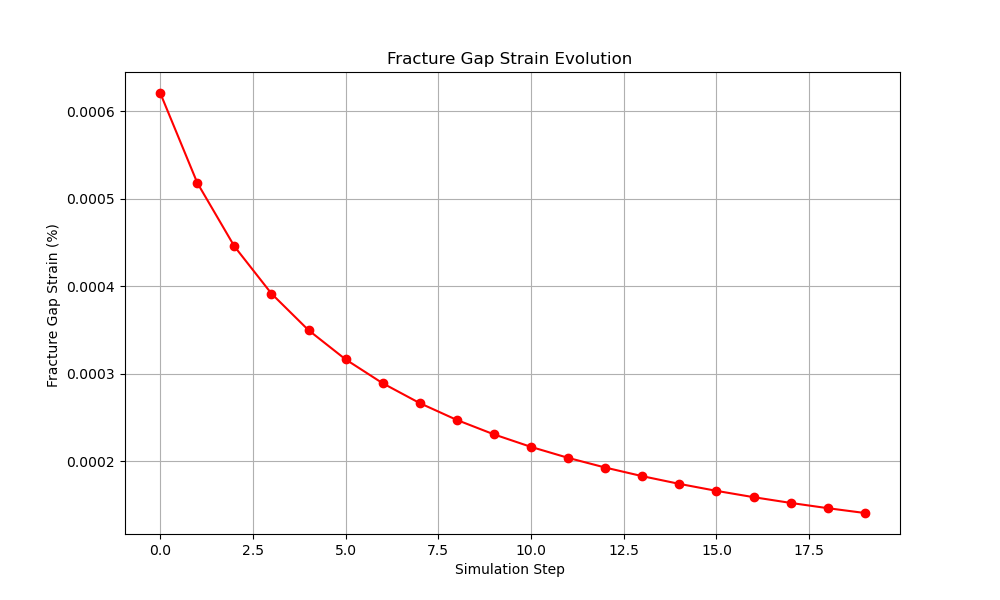
\includegraphics[width=0.7\textwidth]{../output_advanced/Flexible/gap_strain.png}
  \caption{Fracture gap strain evolution over simulation steps for the Flexible Fixator.}
  \label{fig:flexible_gap_strain}
\end{figure}

\begin{figure}[htbp]
  \centering
  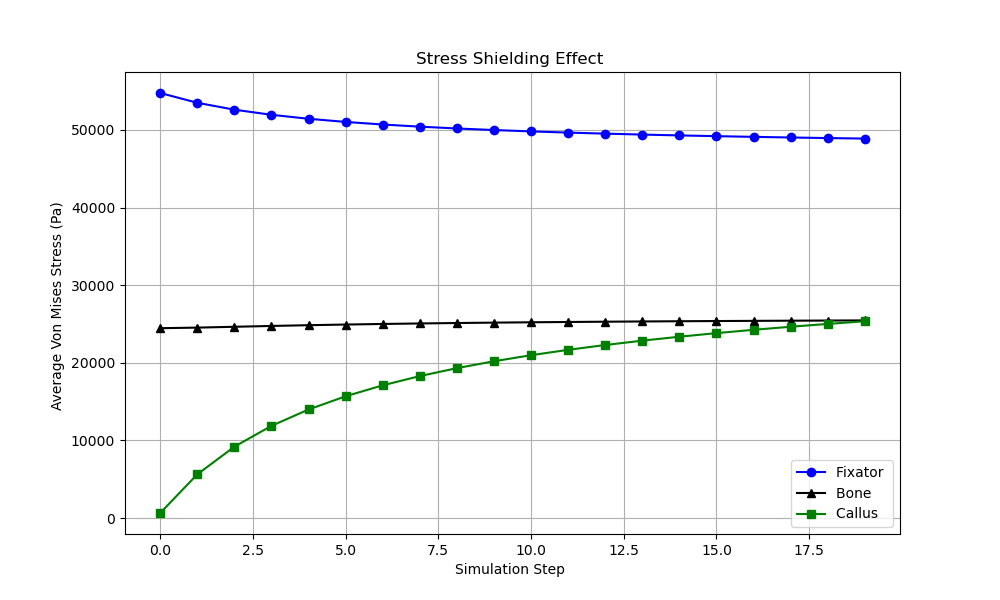
\includegraphics[width=0.7\textwidth]{../output_advanced/Flexible/stress_shielding.png}
  \caption{Stress shielding effect for the Flexible Fixator: Average Von Mises stress in fixator, bone, and callus over simulation steps.}
  \label{fig:flexible_stress_shielding}
\end{figure}

\clearpage % Ensures figures are placed before next major section

\subsection{Standard Fixator (\texorpdfstring{$E_{fixator} = 70$}{E\_fixator = 70} GPa)}

\begin{figure}[htbp]
  \centering
  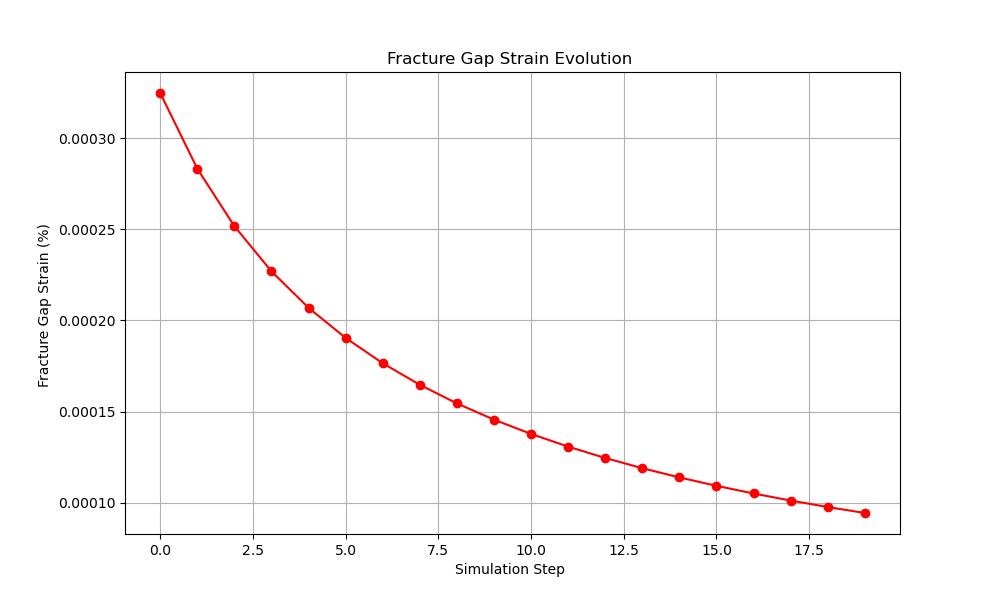
\includegraphics[width=0.7\textwidth]{../output_advanced/Standard/gap_strain.png}
  \caption{Fracture gap strain evolution over simulation steps for the Standard Fixator.}
  \label{fig:standard_gap_strain}
\end{figure}

\begin{figure}[htbp]
  \centering
  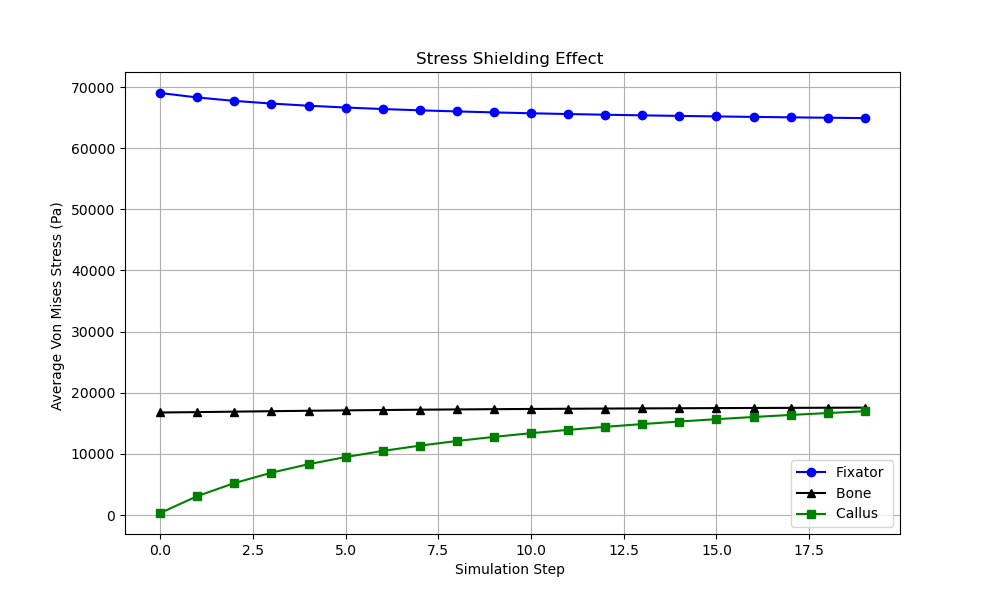
\includegraphics[width=0.7\textwidth]{../output_advanced/Standard/stress_shielding.png}
  \caption{Stress shielding effect for the Standard Fixator: Average Von Mises stress in fixator, bone, and callus over simulation steps.}
  \label{fig:standard_stress_shielding}
\end{figure}

\clearpage % Ensures figures are placed before next major section

\subsection{Rigid Fixator (\texorpdfstring{$E_{fixator} = 140$}{E\_fixator = 140} GPa)}

\begin{figure}[htbp]
  \centering
  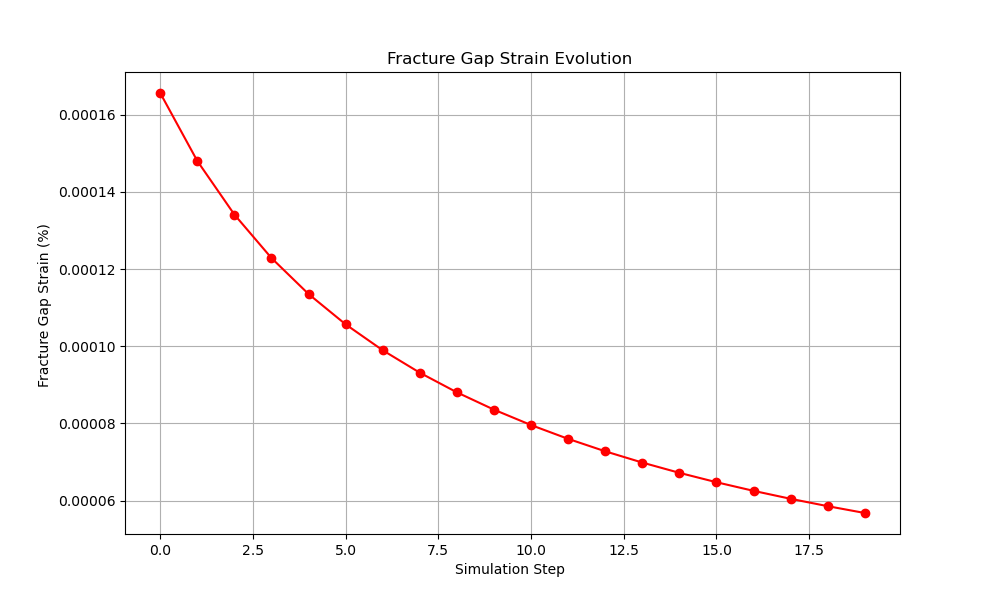
\includegraphics[width=0.7\textwidth]{../output_advanced/Rigid/gap_strain.png}
  \caption{Fracture gap strain evolution over simulation steps for the Rigid Fixator.}
  \label{fig:rigid_gap_strain}
\end{figure}

\begin{figure}[htbp]
  \centering
  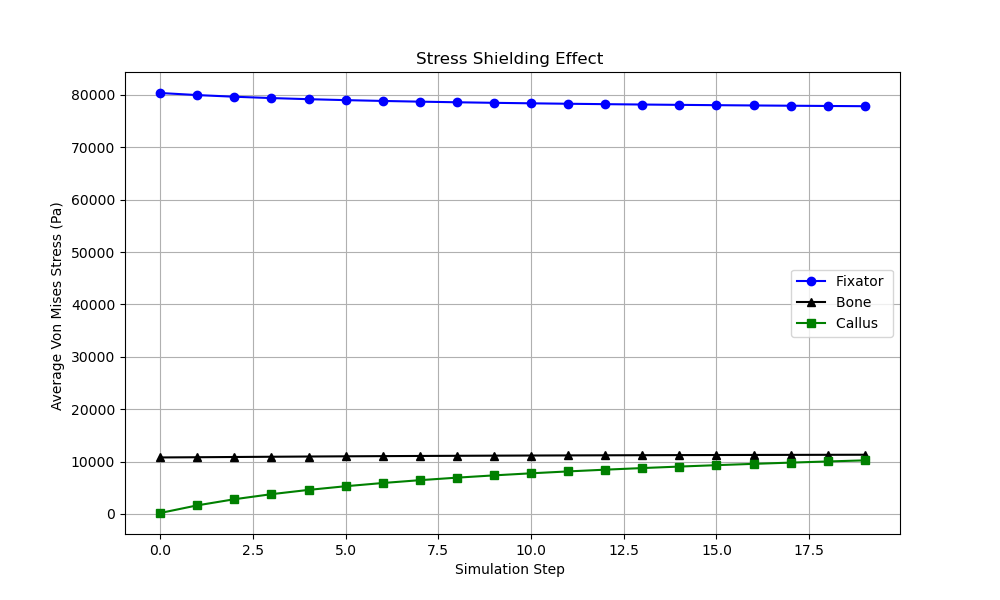
\includegraphics[width=0.7\textwidth]{../output_advanced/Rigid/stress_shielding.png}
  \caption{Stress shielding effect for the Rigid Fixator: Average Von Mises stress in fixator, bone, and callus over simulation steps.}
  \label{fig:rigid_stress_shielding}
\end{figure}

\clearpage

\section{Conclusion}
This project successfully developed and utilized a 2D finite element model to simulate the biomechanics of fracture healing under different fixator stiffnesses. The parametric study demonstrated that:
\begin{itemize}
  \item Increasing fixator stiffness leads to higher stress concentrations in the fixator itself and lower stresses in the bone and healing callus, illustrating the stress shielding phenomenon.
  \item More rigid fixators result in lower fracture gap strains throughout the simulated healing process.
\end{itemize}
These findings align with established biomechanical principles. The flexible fixator allowed for greater load sharing with the bone and callus, potentially promoting more robust healing, while the rigid fixator provided maximum stability but also the most significant stress shielding. The standard fixator offered an intermediate response.

The developed Python scriptprovides a reusable framework for such simulations, allowing for the generation of detailed stress contours, stress/strain evolution plots, and comparative analyses. Figure \ref{fig:parametric_comparison} visually summarizes the key differences observed across the fixator types at the end of the simulated healing period.

Future work could expand this model to 3D, incorporate more complex material models for bone and callus (e.g., anisotropic, viscoelastic), and integrate mechanobiological rules to simulate tissue differentiation directly. Nevertheless, the current model serves as a valuable tool for understanding the fundamental interplay between fixator mechanics and the fracture healing environment.

\begin{figure}[htbp]
  \centering
  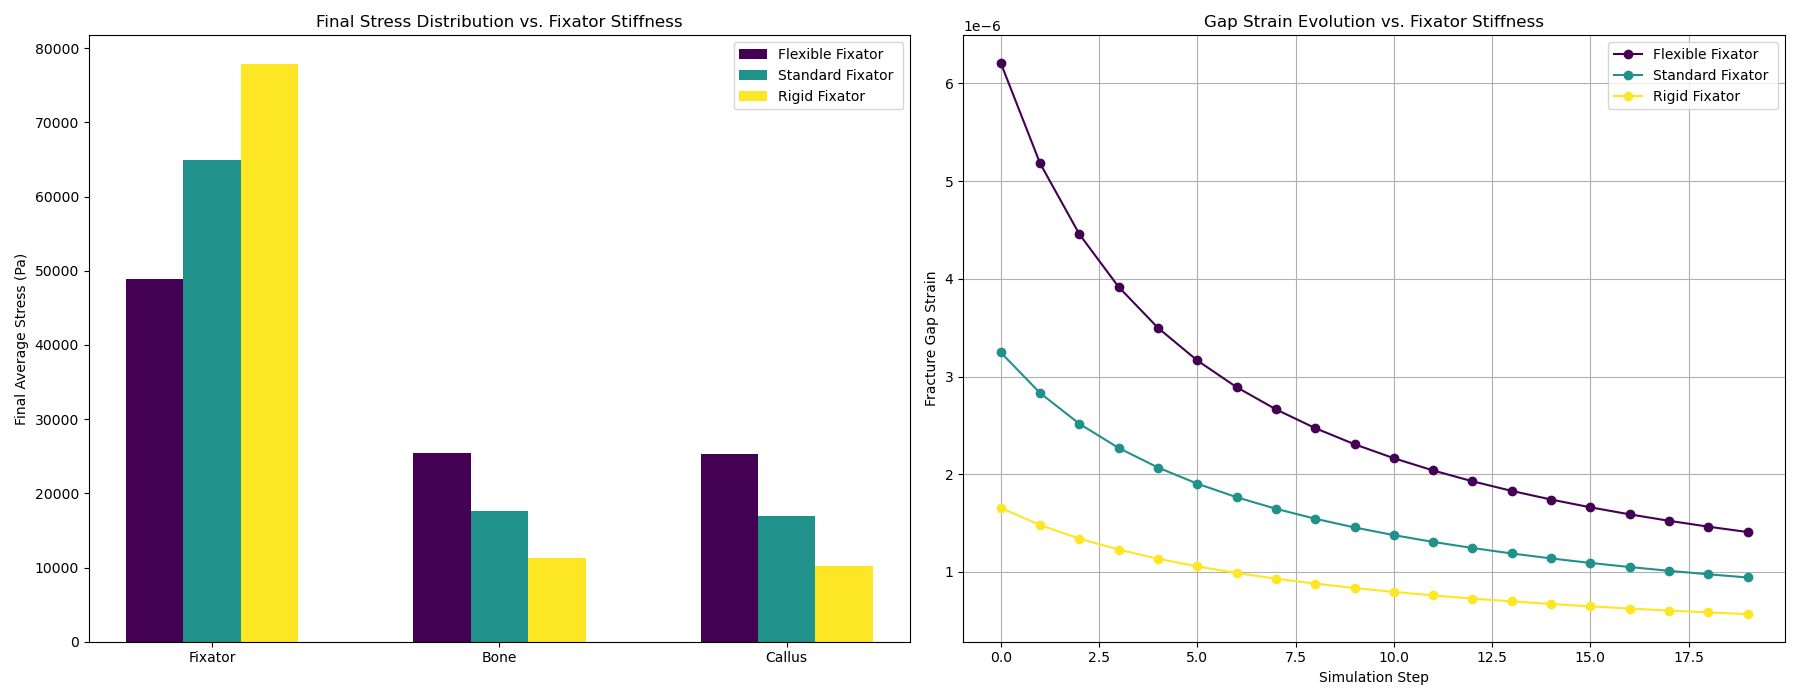
\includegraphics[width=0.95\textwidth]{../output_advanced/parametric_comparison.png}
  \caption{Parametric comparison across different fixator stiffnesses: (Left) Final average Von Mises stress distribution in fixator, bone, and callus. (Right) Fracture gap strain evolution over simulation steps.}
  \label{fig:parametric_comparison}
\end{figure}


%%%%%%%%%%%%%%%%%%%%%%%%%%%%%%%%%%%%%%%%%%%%%%%%%%%%%%%%%%%%%%%%%%%%%%%%%%%%%%%%%%
%%%%%%%%%%%%%%%%%%%%%%%%%%%%%%%%%%%%%%%%%%%%%%%%%%%%%%%%%%%%%%%%%%%%%%%%%%%%%%%%%%

% \section{Introduction}
% \lipsum[2]
% \lipsum[3]


% \section{Headings: first level}
% \label{sec:headings}

% \lipsum[4] See Section \ref{sec:headings}.

% \subsection{Headings: second level}
% \lipsum[5]
% \begin{equation}
% 	\xi _{ij}(t)=P(x_{t}=i,x_{t+1}=j|y,v,w;\theta)= {\frac {\alpha _{i}(t)a^{w_t}_{ij}\beta _{j}(t+1)b^{v_{t+1}}_{j}(y_{t+1})}{\sum _{i=1}^{N} \sum _{j=1}^{N} \alpha _{i}(t)a^{w_t}_{ij}\beta _{j}(t+1)b^{v_{t+1}}_{j}(y_{t+1})}}
% \end{equation}

% \subsubsection{Headings: third level}
% \lipsum[6]

% \paragraph{Paragraph}
% \lipsum[7]



% \section{Examples of citations, figures, tables, references}
% \label{sec:others}

% \subsection{Citations}
% Citations use \verb+natbib+. The documentation may be found at
% \begin{center}
% 	\url{http://mirrors.ctan.org/macros/latex/contrib/natbib/natnotes.pdf}
% \end{center}

% Here is an example usage of the two main commands (\verb+citet+ and \verb+citep+): Some people thought a thing \citep{kour2014real, hadash2018estimate} but other people thought something else \citep{kour2014fast}. Many people have speculated that if we knew exactly why \citet{kour2014fast} thought this\dots

% \subsection{Figures}
% \lipsum[10]
% See Figure \ref{fig:fig1}. Here is how you add footnotes. \footnote{Sample of the first footnote.}
% \lipsum[11]

% \begin{figure}
% 	\centering
% 	\fbox{\rule[-.5cm]{4cm}{4cm} \rule[-.5cm]{4cm}{0cm}}
% 	\caption{Sample figure caption.}
% 	\label{fig:fig1}
% \end{figure}

% \subsection{Tables}
% See awesome Table~\ref{tab:table}.

% The documentation for \verb+booktabs+ (`Publication quality tables in LaTeX') is available from:
% \begin{center}
% 	\url{https://www.ctan.org/pkg/booktabs}
% \end{center}


% \begin{table}
% 	\caption{Sample table title}
% 	\centering
% 	\begin{tabular}{lll}
% 		\toprule
% 		\multicolumn{2}{c}{Part}                   \\
% 		\cmidrule(r){1-2}
% 		Name     & Description     & Size ($\mu$m) \\
% 		\midrule
% 		Dendrite & Input terminal  & $\sim$100     \\
% 		Axon     & Output terminal & $\sim$10      \\
% 		Soma     & Cell body       & up to $10^6$  \\
% 		\bottomrule
% 	\end{tabular}
% 	\label{tab:table}
% \end{table}

% \subsection{Lists}
% \begin{itemize}
% 	\item Lorem ipsum dolor sit amet
% 	\item consectetur adipiscing elit.
% 	\item Aliquam dignissim blandit est, in dictum tortor gravida eget. In ac rutrum magna.
% \end{itemize}


\bibliographystyle{unsrtnat}
\bibliography{references}  %%% Uncomment this line and comment out the ``thebibliography'' section below to use the external .bib file (using bibtex) .


%%% Uncomment this section and comment out the \bibliography{references} line above to use inline references.
% \begin{thebibliography}{1}

% 	\bibitem{kour2014real}
% 	George Kour and Raid Saabne.
% 	\newblock Real-time segmentation of on-line handwritten arabic script.
% 	\newblock In {\em Frontiers in Handwriting Recognition (ICFHR), 2014 14th
% 			International Conference on}, pages 417--422. IEEE, 2014.

% 	\bibitem{kour2014fast}
% 	George Kour and Raid Saabne.
% 	\newblock Fast classification of handwritten on-line arabic characters.
% 	\newblock In {\em Soft Computing and Pattern Recognition (SoCPaR), 2014 6th
% 			International Conference of}, pages 312--318. IEEE, 2014.

% 	\bibitem{hadash2018estimate}
% 	Guy Hadash, Einat Kermany, Boaz Carmeli, Ofer Lavi, George Kour, and Alon
% 	Jacovi.
% 	\newblock Estimate and replace: A novel approach to integrating deep neural
% 	networks with existing applications.
% 	\newblock {\em arXiv preprint arXiv:1804.09028}, 2018.

% \end{thebibliography}


\end{document}
